\documentclass[a4paper,12pt]{article} % добавить leqno в [] для нумерации слева
\usepackage[a4paper,top=1.3cm,bottom=2cm,left=1.5cm,right=1.5cm,marginparwidth=0.75cm]{geometry}
%%% Работа с русским языком
\usepackage{cmap}					% поиск в PDF
\usepackage{mathtext} 				% русские буквы в фомулах
\usepackage[T2A]{fontenc}			% кодировка
\usepackage[utf8]{inputenc}			% кодировка исходного текста
\usepackage[english,russian]{babel}	% локализация и переносы

\usepackage{graphicx}

\usepackage{wrapfig}
\usepackage{tabularx}

\usepackage{hyperref}
\usepackage[rgb]{xcolor}
\hypersetup{
colorlinks=true,urlcolor=blue
}
\usepackage{multirow}
\usepackage{hhline}


%%% Дополнительная работа с математикой
\usepackage{amsmath,amsfonts,amssymb,amsthm,mathtools} % AMS
\usepackage{icomma} % "Умная" запятая: $0,2$ --- число, $0, 2$ --- перечисление

%% Номера формул
\mathtoolsset{showonlyrefs=true} % Показывать номера только у тех формул, на которые есть \eqref{} в тексте.

%% Шрифты
\usepackage{euscript}	 % Шрифт Евклид
\usepackage{mathrsfs} % Красивый матшрифт

%% Свои команды
\DeclareMathOperator{\sgn}{\mathop{sgn}}

%% Перенос знаков в формулах (по Львовскому)
\newcommand*{\hm}[1]{#1\nobreak\discretionary{}
{\hbox{$\mathsurround=0pt #1$}}{}}

\begin{document}
	
	\begin{titlepage}
	\begin{center}
		{\large МОСКОВСКИЙ ФИЗИКО-ТЕХНИЧЕСКИЙ ИНСТИТУТ (НАЦИОНАЛЬНЫЙ ИССЛЕДОВАТЕЛЬСКИЙ УНИВЕРСИТЕТ)}
	\end{center}
	\begin{center}
		{\large Физтех-школа электроники, фотоники и молекулярной физики}
	\end{center}
	
	
	\vspace{4.5cm}
	{\huge
		\begin{center}
			{Лабораторная работа 2.5.1}\\
			Измерение коэффициента поверхностного натяжения жидкости
		\end{center}
	}
	\vspace{2cm}
	\begin{flushright}
		{\LARGE Салтыкова Дарья \\
			\vspace{0.5cm}
			Б04-105}
	\end{flushright}
	\vspace{8cm}
	\begin{center}
		Долгопрудный 2022
	\end{center}
\end{titlepage}

\section{Введение}

\textbf{Цель работы:} 1) измерение температурной зависимости  коэффициента поверхностного натяжения дистиллированной воды с использованием известного коэффициента поверхностного натяжения спирта;  2) определение полной поверхностной энергии  и теплоты, необходимой для изотермического образования единицы  поверхности жидкости  при различной температуре. 
\medskip

\noindent \textbf{Оборудование:} прибор  Ребиндера  с термостатом и микроманометром; исследуемые жидкости; стаканы.
\medskip

\section{Теоретические сведения}

Наличие поверхностного слоя приводит к различию давлений по разные стороны от искривленной границы раздела двух сред.  Для сферического пузырька с воздухом  внутри жидкости избыточное давление даётся формулой Лапласа:

\begin{equation}
\Delta P = P_{\text{внутри}} - P_{\text{снаружи}} =  \frac{2\sigma}{r} ,
\end{equation}

\noindent где $\sigma$ – коэффициент поверхностного натяжения, $P_{\text{внутри}$ и $P_{\text{снаружи}}$ – давление внутри пузырька и снаружи, $r$ – радиус кривизны поверхности раздела двух фаз. Эта формула лежит в основе предлагаемого метода определения коэффициента поверхностного натяжения жидкости. Измеряется давление $\Delta P$, необходимое для выталкивания в жидкость пузырька воздуха.

\medskip

\section{Экспериментальная установка}

\begin{figure}[h]
\center{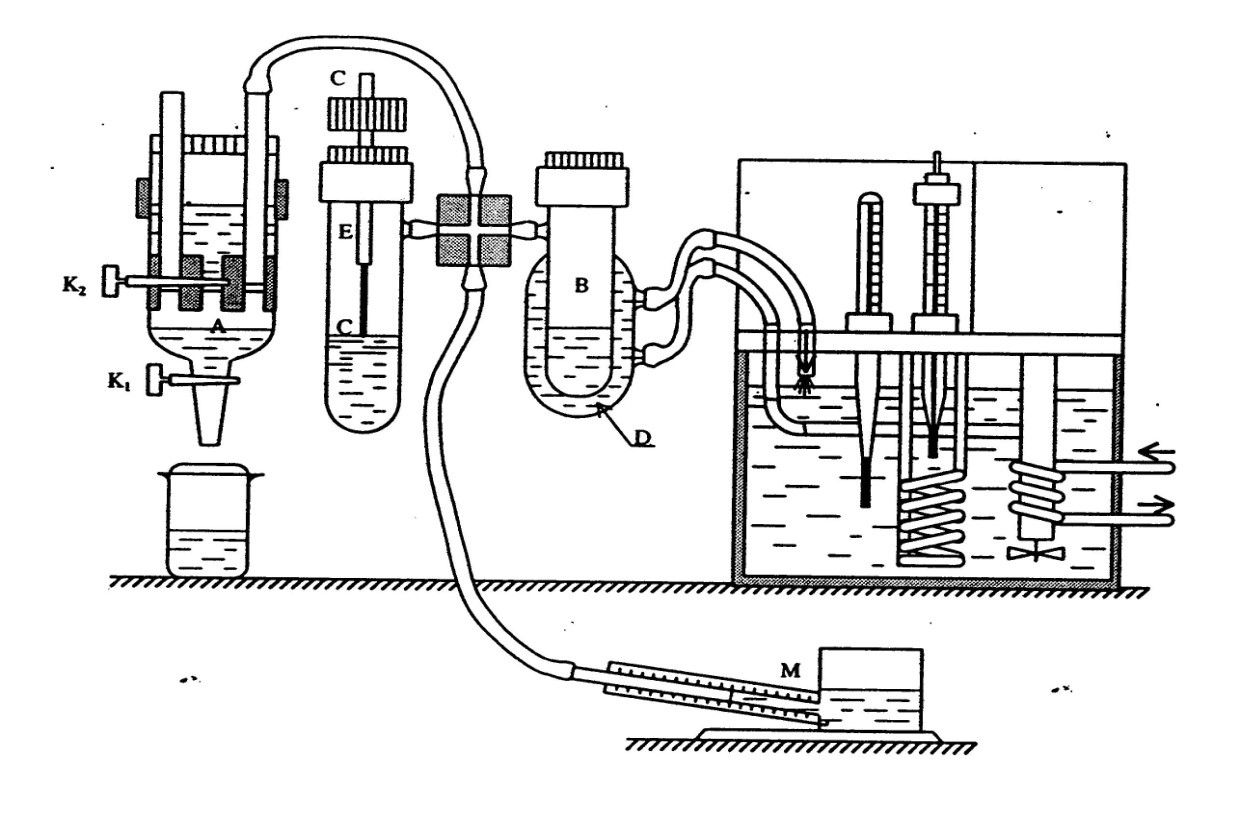
\includegraphics[scale={0.7}]{установка.jpg}}
\caption{Схема установки для измерения температурной зависимости коэффициента поверхностного натяжения.}
\label{fig:image}
\end{figure}

\medskip

\noindent Исследуемая жидкость (дистиллированная вода) наливается в сосуд (колбу) В (Рис.1). Тестовая жидкость  (этиловый спирт) наливается  в сосуд $E$.  При измерениях  колбы герметично закрываются  пробками.   Через одну из двух пробок  проходит полая металлическая игла $C$. Этой пробкой закрывается сосуд, в котором  проводятся измерения. Верхний конец иглы открыт в атмосферу, а нижний погружен в жидкость. Другой сосуд герметично закрывается второй пробкой. При создании достаточного  разряжения воздуха в колбе с иглой пузырьки воздуха начинают пробулькивать через жидкость. Поверхностное натяжение можно определить по величине разряжения $\Delta P$, необходимого для прохождения пузырьков (при известном радиусе иглы).

\medskip

\noindent Разряжение в системе создается с помощью аспиратора $A$. Кран $K_{2}$ разделяет две полости аспиратора. Верхняя полость при закрытом кране $K_{2}$  заполняется водой. Затем кран $K_{2}$ открывают и заполняют водой  нижнюю полость  аспиратора.  Разряжение воздуха создается в нижней полости  при открывании крана $K_{1}$, когда  вода вытекает из неё по каплям. В колбах $B$ и $C$, соединённых трубками с нижней полостью аспиратора,  создается такое же пониженное давление. Разность давлений в полостях с разряженным воздухом и атмосферой измеряется спиртовым микроманометром.

\medskip
 
\noindent Для стабилизации температуры исследуемой жидкости через рубашку $D$ колбы $B$ непрерывно прогоняется вода из термостата.

\medskip

\noindent Обычно кончик иглы лишь касается поверхности жидкости, чтобы исключить влияние гидростатического давления столба жидкости. Однако при измерении температурной зависимости коэффициента поверхностного натяжения возникает ряд сложностей. Во-первых, большая теплопроводность металлической трубки приводит к тому, что температура на конце трубки заметно ниже, чем в глубине жидкости. Во-вторых, тепловое расширение поднимает уровень жидкости при увеличении температуры. 

\medskip

\noindent Обе погрешности можно устранить, погрузив кончик трубки до самого дна. Полное давление, измеренное при этом микроманометром, $P = \Delta P + \rho gh$. Заметим, что $\rho gh$ от температуры практически не зависит, так как подъём уровня жидкости компенсируется уменьшением её плотности (произведение $\rho h$ определяется массой всей жидкости и поэтому постоянно). Величину  $\rho gh$ следует измерить двумя способами. Во-первых, замерить величину $P_{1}= \Delta P^\prime$, когда кончик трубки только касается поверхности жидкости. Затем при этой же температуре опустить иглу до дна и замерить $P_{2}= \rho gh + \Delta P^{\prime\prime} (\Delta P^\prime, \Delta P^{\prime\prime}$ – давление Лапласа). Из-за  несжимаемости  жидкости можно положить $\Delta P^\prime = \Delta P^{\prime\prime}$ и тогда $\rho gh = P_{2} - P_{1}$. Во-вторых, при измерениях $P_{1}$ и $P_{2}$ замерить линейкой  глубину погружения иглы $h$. Это можно сделать, замеряя расстояние между верхним концом иглы и любой неподвижной частью прибора при положении иглы на поверхности и в глубине колбы.
Замечание. Чувствительность микроманометра высока, поэтому правильность его работы существенно зависит от правильности  эксплуатации прибора. Все изменения в установке необходимо проводить, предварительно поставив переключатель микроманометра на атмосферу.

\medskip

\noindent В частности подобную же операцию необходимо сделать и при заполнении водой аспиратора $A$. В противном случае при заполнении аспиратора водой давление воздуха в системе повышается, спирт из трубки микроманометра выдавливается, в узлах соединений микроманометра образуются воздушные пузыри. Наличие этих пузырей приводит к полному нарушению калибровки манометра и невоспроизводимости измерений.

\medskip

\section{Ход работы}

1. Проверим герметичность установки. Для этого заполним аспиратор водой. Чистую сухую иглу установим в сосуд со спиртом так, чтобы кончик иглы лишь касался поверхности спирта. Плотно закроем обе колбы $B$ и $E$ пробками. Откроем кран $K_{1}$ аспиратора и добьемся пробулькивания пузырьков воздуха в колбе. Замерим показания микроманометра. Закроем кран $K_{1}$. Наблюдаем за показаниями манометра: столбик спирта в манометре неподвижен - течь в устновке отсутствует.

\medskip
 

\noindent 2. Проведем измерения для спирта. Подберем частоту падения капель из аспиратора так, чтобы максимальное давление манометра не зависело от этой частоты (примерно 1 капля в 5 секунд) Измерим максимальное давление $\Delta P_{\text{спирта}}$ при  пробулькивании пузырьков воздуха через спирт.

\begin{tabular}{|c|c|c|c|c|c|}
\hline 
№ & 1 & 2 & 3 & 4 & 5 \\ 
\hline 
$\Delta{P_{\text{спирта}}}$, мм вод ст & 42 & 43 & 42 & 42 & 43 \\ 
\hline 
$\Delta{P_{\text{спирта}}}$, Па & 82,4 & 84,3 & 82,4 & 82,4 & 84,3 \\ 
\hline 
$\langle \Delta{P_{\text{спирта}}} \rangle$, Па & \multicolumn{5}{c|}{82,8} \\ 
\hline 
$ \sigma_{P} $, Па  & \multicolumn{5}{c|}{2,0} \\ 
\hline 
\end{tabular} 

\medskip

\noindent Cлучайную погрешность измерений оценим по формуле

\begin{equation}
\sigma_{P}^{\text{случ}} = \sqrt{\frac{1}{N(N-1)}\sum\limits_{k=1}^N\left(\Delta{P_{\text{спирта}}}_k-\langle \Delta{P_{\text{спирта}}} \rangle\right)^2} \approx 0,5 \text{ Па}.
\end{equation}

\medskip

\noindent Будем считать, что систематическая погрешность измерения составила $ 1 $ мм вод ст, т. е. {$ \sigma_{P}^\text{сист} \approx 1,9 $ Па}.

\medskip

\noindent Полная погрешность измерений определяется по формуле:

\begin{equation}
\sigma_{P}=\sqrt{(\sigma_{P}^\text{сист})^2 + (\sigma_{P}^\text{случ})^2} \approx 2,0 \text{ Па}.
\end{equation}

\medskip

\noindent Итого { $ \Delta P_{\text{спирта}} = (82,8 \pm 2,0) \text{ Па},$} \quad $(\varepsilon_{\Delta P_{\text{спирта}}} = 2,4 \%) $.

\medskip

\noindent 3. Вытащим иглу, просушим ее и измерим микроскопом ее диаметр:

\medskip

\begin{tabular}{|c|c|c|c|c|c|}
\hline 
№ & 1 & 2 & 3 & 4 & 5 \\ 
\hline 
$d$, мм & 1 & 0,9 & 0,9 & 0,8 & 0,9 \\ 
\hline 
$\langle d \rangle$, мм & \multicolumn{5}{c|}{0,9} \\ 
\hline 
$\sigma_{d}$, мм & \multicolumn{5}{c|}{0,06} \\ 
\hline 
\end{tabular} 

\medskip

\noindent Cлучайную погрешность измерений оценим по формуле

\medskip

\begin{equation}
\sigma_{d}^{\text{случ}} = \sqrt{\frac{1}{N(N-1)}\sum\limits_{k=1}^N\left(d_k-\langle d \rangle\right)^2} \approx 0,03 \text{ мм}.
\end{equation}

\medskip

\begin{equation}
\sigma_{d}^\text{сист} \approx 0,05 \text{ мм}
\end{equation}

\medskip

\begin{equation}
\sigma_{d}=\sqrt{(\sigma_{d}^\text{сист})^2 + (\sigma_{d}^\text{случ})^2} \approx 0,06 \text{ мм}.
\end{equation}

\medskip

\noindent Получаем { $d = (0,9 \pm 0,06) \text{ мм},$} $(\varepsilon_d = 6,6 \%) $.

\medskip

\noindent Из табличного значения коэффициента поверхностного натяжения спирта $\sigma = 22,4 \text{мН/м}$ получим:

\medskip

\begin{equation}
d = \frac{4\sigma}{\Delta P} = 1,08\text{ мм}
\end{equation}

\medskip

\begin{equation}
\sigma_d=d \varepsilon_{\Delta P} \approx 0,03 \text{ мм}.
\end{equation}

\medskip

\noindent Получаем { $d = (1,08 \pm 0,03) \text{ мм},$} $(\varepsilon_d = 2,7 \%) $.

\medskip

\noindent Таким образом, в пределах погрешности диаметры иглы, измеренные разными способами, совпадают.

\medskip


\noindent 4. Перенесем предварительно промытую и просушенную от спирта иглу в колбу с дистиллированной водой. Измерим максимальное давление $P_{1}$ при пробулькивании пузырьков, когда игла лишь касается поверхности воды.

\medskip

\begin{tabular}{|c|c|c|c|c|c|}
\hline 
№ & 1 & 2 & 3 & 4 & 5 \\ 
\hline 
$P_{1}$, мм вод ст & 133 & 133 & 132 & 133 & 134 \\ 
\hline 
$P_{1}$, Па & 261 & 261 & 259 & 261 & 263 \\ 
\hline 
$\langle P_{1} \rangle$, Па & \multicolumn{5}{c|}{261} \\ 
\hline 
$\sigma_{P_{1}} $, Па  & \multicolumn{5}{c|}{2,00} \\ 
\hline 
\end{tabular} 

\medskip

\noindent Измерим расстояние между верхним концом иглы и неподвижной частью прибора $h_{1}$.

\medskip

\begin{tabular}{|c|c|c|c|c|c|}
\hline 
№ & 1 & 2 & 3 & 4 & 5 \\ 
\hline 
$h_{1}$, мм & 48 & 47 & 48 & 47 & 47 \\ 
\hline 
$\langle h_{1} \rangle$, мм & \multicolumn{5}{c|}{47,40} \\ 
\hline 
$\sigma_{h_{1}}$, мм & \multicolumn{5}{c|}{1,03} \\ 
\hline 
\end{tabular} 

\medskip


\noindent Утопим иглу до предела. Измерим максимальное давление в пузырьках $P_{2}$.

\medskip

\begin{tabular}{|c|c|c|c|c|c|}
\hline 
№ & 1 & 2 & 3 & 4 & 5 \\ 
\hline 
$P_{2}$, мм вод ст & 210 & 208 & 209 & 209 & 208 \\ 
\hline 
$P_{2}$, Па & 412 & 408 & 410 & 410 & 408 \\ 
\hline 
$\langle P_{2} \rangle$, Па & \multicolumn{5}{c|}{409,6} \\ 
\hline 
$\sigma_{P_{2}} $, Па  & \multicolumn{5}{c|}{2,0} \\ 
\hline 
\end{tabular}

\medskip

\noindent Измерим $h_{2}$.

\medskip

\begin{tabular}{|c|c|c|c|c|c|}
\hline 
№ & 1 & 2 & 3 & 4 & 5 \\ 
\hline 
$h_{2}$, мм & 64 & 65 & 66 & 65 & 65 \\ 
\hline 
$\langle h_{2} \rangle$, мм & \multicolumn{5}{c|}{65} \\ 
\hline 
$\sigma_{h_{2}}$, мм & \multicolumn{5}{c|}{1} \\ 
\hline 
\end{tabular} 

\medskip

\noindent По полученным данным определяем

\medskip
 
\begin{equation}
\Delta P = P_2 - P_1 = 148,6 \text{ Па}
\end{equation}

\medskip

\begin{equation}
\sigma_{\Delta P} = \sqrt{\sigma^2_{P_1}+\sigma^2_{P_2}} \approx 2,8 \text{ Па}, (\varepsilon_{\Delta P} = 0,02\text{ Па})
\end{equation}

\medskip

\begin{equation}
\Delta h = h_{1} - h_{2} = 17,6 \text{ мм}
\end{equation}
 
\medskip

\begin{equation}
\sigma_{\Delta h} = \sqrt{\sigma^2_{h_1}+\sigma^2_{h_2}} \approx 1,4 \text{ мм}
\end{equation}

\medskip
\noindent Получим { $\Delta h = (17,6 \pm 1,4) \text{ мм},$} $(\varepsilon_{\Delta h} = 7,9 \%) $.
\medskip

\noindent По полученному значению $\Delta P$ вычислим $\Delta h$:

\medskip
 
\begin{equation}
\Delta h = \frac{\Delta P}{\rho g} = 18,2 \text{ мм}, 
\end{equation}

\medskip

\noindent где $\rho = 0,8095$ г/м^3 - $\text{ плотность этилового спирта при данной температуре}$.

\medskip

\begin{equation}
\sigma_{\Delta h} = \Delta h \varepsilon_{\Delta P} \approx 0,3 \text{ мм}
\end{equation}

\medskip

\noindent Итого { $\Delta h = (18,2 \pm 0,3) \text{ мм},$} $(\varepsilon_{\Delta h} = 1,6 \%) $.

\medskip

\noindent Таким образом, в пределах погрешности $\Delta h$, вычисленные прямо и косвенно, совпадают.

\medskip

\noindent 5. Снимем температурную зависимость $\sigma (T)$ дистиллированной воды. При измерении давления будем делать поправку на добавочное давление со стороны столба жидкости, полученную в предыдущем пункте: {$\Delta P = (148,6 \pm 0,02) \text{ Па}.$}
\medskip

\begin{tabular}{|c|c|c|c|c|c|c|c|c|}
\hline 
$T, ^\circ\text{C}$ & 24 & 30 & 35 & 40 & 45 & 50 & 55 & 60 \\ 
\hline 
 & 210 & 207 & 203 & 200 & 199 & 198 & 197 & 194 \\ 
\hhline{~--------} 
 $P', \text{мм вод ст}$ & 208 & 206 & 203 & 200 & 200 & 198 & 197 & 195 \\ 
\hhline{~--------} 
 $\text{(без учета } \Delta P \text{)}$ & 209 & 207 & 202 & 200 & 199 & 198 & 197 & 195 \\ 
\hhline{~--------} 
 & 209 & 207 & 203 & 200 & 199 & 198 & 196 & 196 \\ 
\hhline{~--------} 
 & 208 & 206 & 203 & 199 & 199 & 198 & 197 & 196 \\ 
\hline 
$\langle P \rangle, \text{Па}$ & 261 & 256 & 249 & 244 & 242 & 241 & 238 & 234 \\ 
\hline 
$\sigma_{P}, \text{Па}$ & 2,0 & 2,0 & 1,9 & 1,9 & 1,9 & 0 & 1,9 & 2,1 \\ 
\hline 
$\sigma, \text{мН/м}$ & 70,5 & 69,2 & 67,2 & 65,8 & 65,3 & 65,1 & 64,3 & 63,2 \\ 
\hline 
$\sigma_{\sigma}, \text{мН/м}$ & 1,5 & 1,5 & 1,4 & 1,4 & 1,4 & 1,5 & 1,5 & 1,4 \\ 
\hline 
\end{tabular} 

\medskip
\medskip

\noindent Вычислим коэффициент поверхностного натяжения для каждой из температур по формуле

\medskip

\begin{equation}
\sigma = \frac{Pd}{4},
\end{equation}

\medskip

\noindent где $ d $ -- диаметр иглы. 

\noindent Погрешность вычисляется по следующей формуле:

\begin{equation}
\sigma_\sigma = \sigma\sqrt{\varepsilon^2_P + \varepsilon^2_d}.
\end{equation}
\medskip

\noindent Полученную зависимость нанесем на график. 

\begin{figure}[h!]
\center{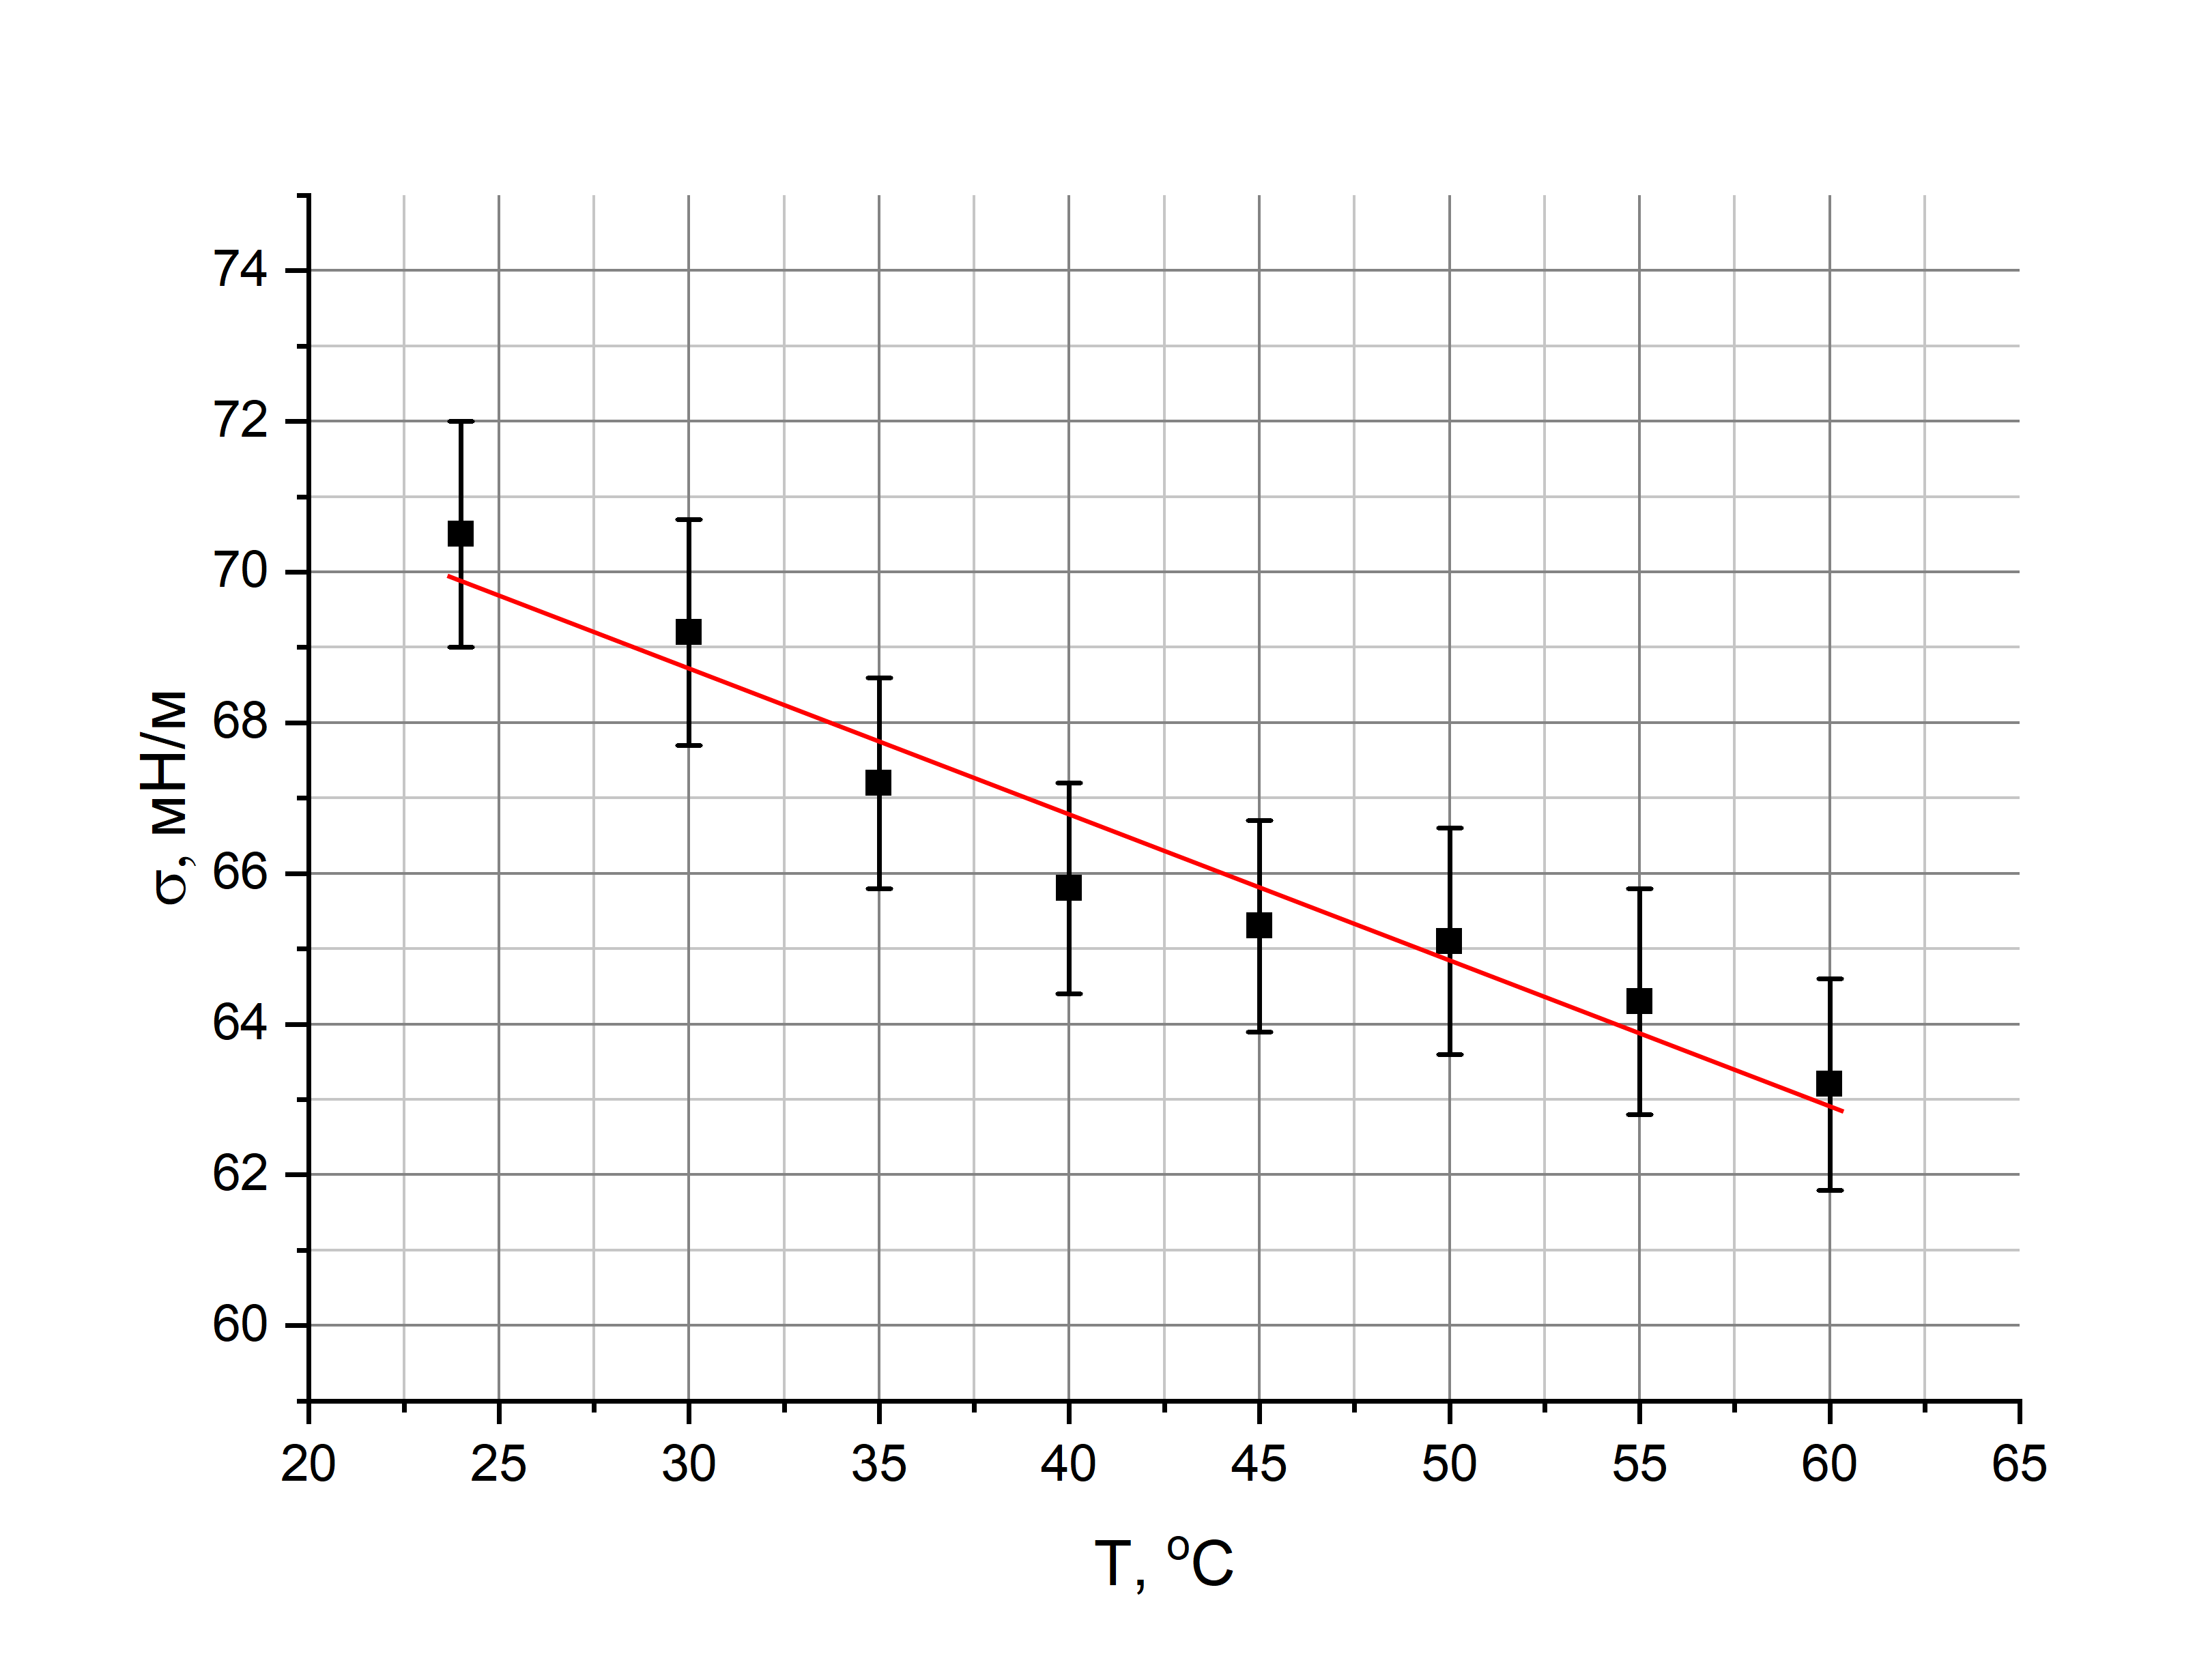
\includegraphics[scale={0.5}]{1.png}}
\end{figure}

\medskip

\noindent Вычислим коэффициенты аппроксимирующей прямой $ \sigma = kT + b $, где $ \displaystyle k = \frac{d\sigma}{dT} $, используя метод наименьших квадратов:

\medskip

\[ k = \frac{\langle T\sigma \rangle - \langle T \rangle \langle \sigma \rangle}{\langle T^2 \rangle - \langle T \rangle ^2} \approx -0,194\text{ } \frac{\text{мН}}{\text{м}\cdot\text{К}},\]

\medskip

\[ b = \langle \sigma \rangle - k\langle T \rangle \approx 74,5\text{ } \frac{\text{мН}}{\text{м}}. \]

\medskip

\noindent Случайные погрешности оценим по следующим формулам:

\medskip

\[ \sigma^\text{случ}_k = \sqrt{\frac{1}{N-2} \left(\frac{\left\langle\left(\sigma - \langle \sigma\right\rangle\right)^2 \rangle}{\left\langle\left(T - \langle T\right\rangle\right)^2 \rangle}\right)-k^2} \approx 0,008 \text{ } \frac{\text{мН}}{\text{м}\cdot\text{К}},\]

\medskip

\[ \sigma^\text{случ}_b=\sigma^\text{случ}_k\sqrt{\left\langle T^2 \right\rangle - {\langle T \rangle}^2} \approx 1,6\text{ } \frac{\text{мН}}{\text{м}}. \]

\medskip

\noindent Систематические погрешности оценим по следующим формулам:

\medskip

\[ \sigma^\text{сист}_k = |k|\sqrt{\varepsilon^2_T+\varepsilon^2_\sigma} \approx 0,004 \text{ } \frac{\text{мН}}{\text{м}\cdot\text{К}}, \]
\[ \sigma^\text{сист}_b = |b|\sqrt{\varepsilon^2_T+\varepsilon^2_\sigma} \approx 3,2 \text{ } \frac{\text{мН}}{\text{м}}. \]

\medskip


\noindent Тогда полные погрешности составляют:

\medskip

\[ \sigma_k = \sqrt{(\sigma_k^\text{сист})^2 + (\sigma_k^\text{случ})^2} \approx 0,009 \text{ } \frac{\text{мН}}{\text{м}\cdot\text{К}},\]
\[ \sigma_b = \sqrt{(\sigma_b^\text{сист})^2 + (\sigma_b^\text{случ})^2} \approx 3,6 \text{ } \frac{\text{мН}}{\text{м}}. \]

\medskip

\noindent Окончательно:

\medskip

	 $ \displaystyle {k = \frac{d\sigma}{dT} = (-0,194 \pm 0,009) \text{ } \frac{\text{мН}}{\text{м}\cdot\text{К}}, \: (\varepsilon = 4,6\%);} $
	 $ \displaystyle {b = (74,5 \pm 3,6) \text{ } \frac{\text{мН}}{\text{м}}, \: (\varepsilon = 4,8\%).}$


\medskip


\noindent Построим графики зависимости от температуры теплоты образования единицы поверхности жидкости $ \displaystyle {q = -T\frac{d\sigma}{dT}} $ и поверхностной энергии $ U $ единицы площади $ F $: $ \displaystyle {\frac{U}{F} = \left(\sigma - T \frac{d\sigma}{dT}\right).} $


\begin{minipage}{.50\textwidth}
  \centering
  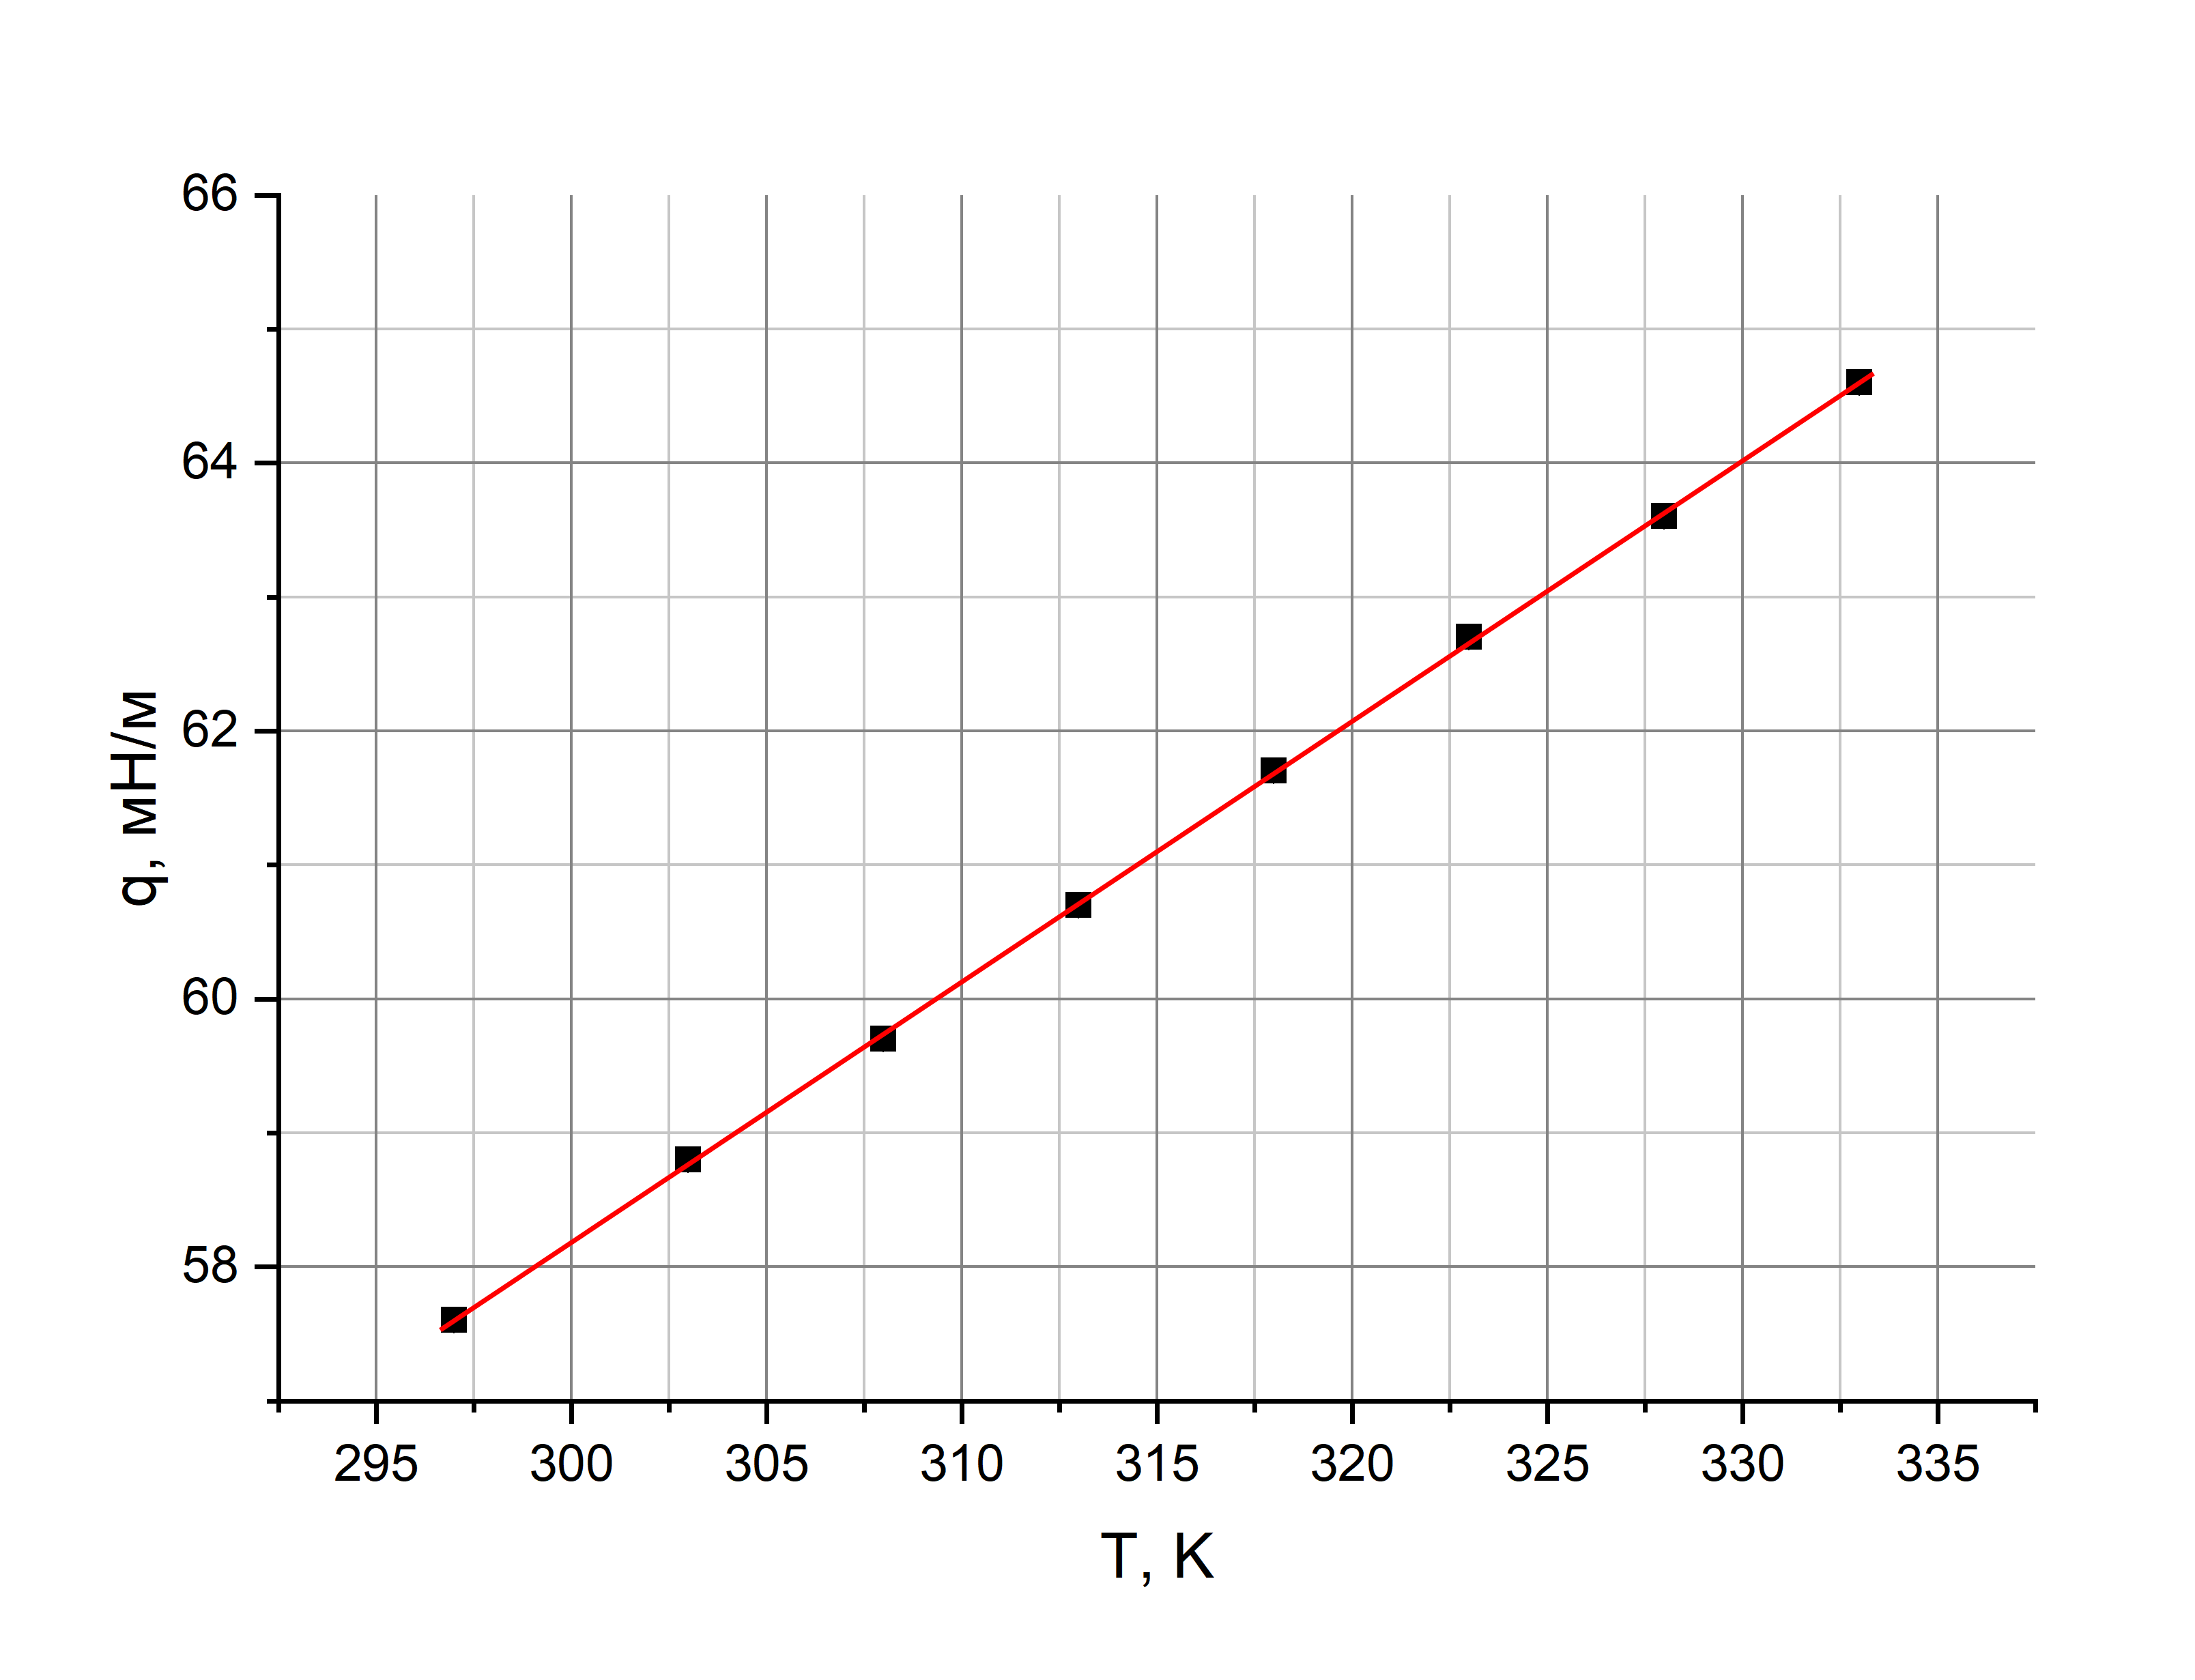
\includegraphics[scale={0.38}]{2.png}
\end{minipage}
\begin{minipage}{.50\textwidth}
  \centering
  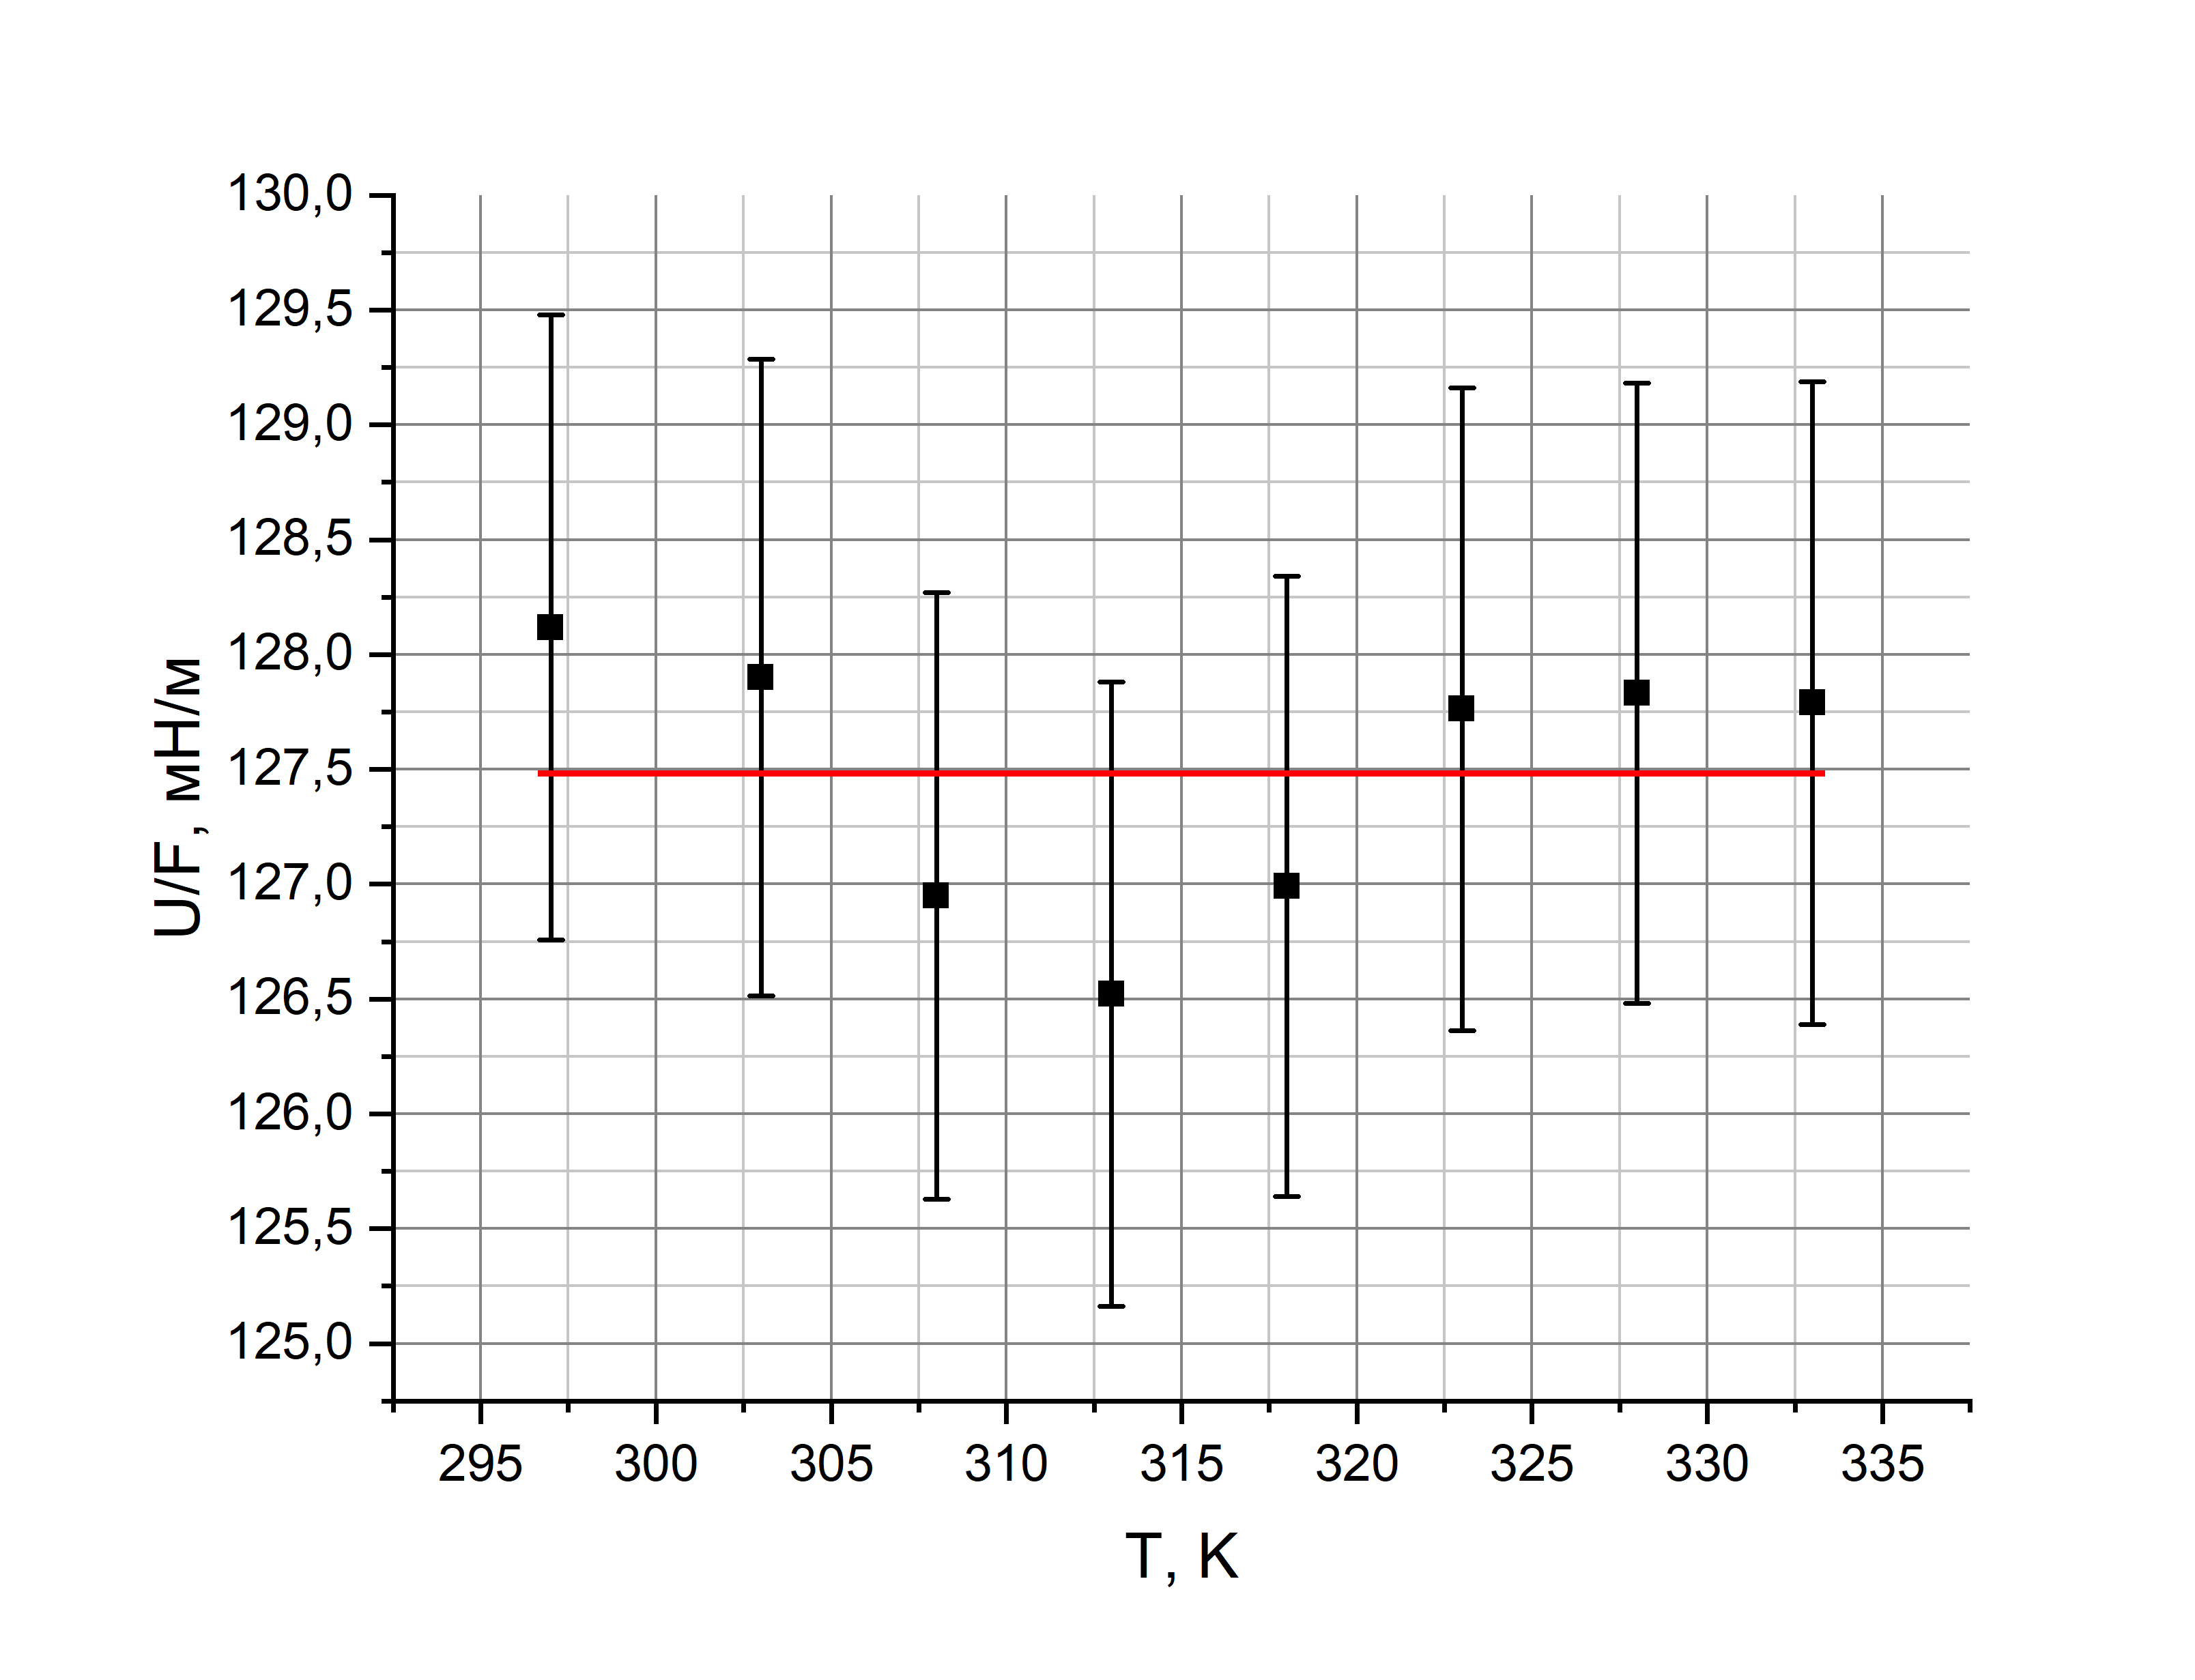
\includegraphics[scale={0.38}]{3.png}
\end{minipage}


\newpage
\section{Вывод}

\medskip

\noindent В ходе работы:

\begin{itemize}
	\item Был получен диаметр иглы двумя способами: с использованием табличного значения коэффициента поверхностного натяжения спирта (${ d = (1,08 \pm 0,03) \text{ мм},} \: (\varepsilon = 2,7\%)$) и с помощью микроскопа (${ d = (0,90 \pm 0,06) \text{ мм},} \: (\varepsilon = 6,6\%)$). В пределах погрешности результаты совпадают.
	
	\item Был экспериментально получен коэффициент поверхностного натяжения воды при различных её температурах, построен график зависимости коэффициента поверхностного натяжения воды от температуры (коэффициент пропорциональности линейной зависимости $\displaystyle {k = \frac{d\sigma}{dT} = (-0,194 \pm 0,009) \text{ } \frac{\text{мН}}{\text{м}\cdot\text{К}},} \: (\varepsilon = 4,6\%) $ ).
	
	\item Были построены графики зависимости от температуры теплоты образования единицы поверхности жидкости и поверхностной энергии единицы площади.
\end{itemize}

\noindent Полученные значения коэффициента поверхностного натяжения воды почти совпадают с табличными данными. Незначительную неточность можно объяснить несовершенной чистотой дистиллята. 	
	
	
\end{document}